% !TEX root = main.tex

% TODO:
% REMARK:

\section{ Systematic Uncertainty}
\label{sec:Systematic}

	Besides the statistical uncertainty, there are also some systematic uncertainty from detector's issue, reconstruction procedure, simulating process...etc. In this snalysis, the primary systematic uncertainties are from the simulation correction. 

	\subsection{Introduction of systematic uncertainty}
	\label{ssec:Syst_type}
		\subsubsection{Pileup re-weighting}
		\label{sssec:Syst_PU}

			% https://twiki.cern.ch/twiki/bin/viewauth/CMS/PileupMCReweightingUtilities?fbclid=IwAR0SuZFQ5Um0IfZn1-CHXia6NPMYe2_7cz2OGXxhCYvNvfl_tTBke-w22l8

			Since the pileup performance under data and simulation(MC) have discrepancy, there is MC reweighing of pileup in any events which is mentioned in section.\ref{sssec:DataAndMC_PU}. However, there is also an uncertainty of pileup reweight. The pp inelastic scattering cross section is used to calculate the pileup distribution and then used to implement the pileup reweight, so this cross section has its mean value and uncertainty 69.2$mb^{-1}$ $\pm$5\%. Then the pileup reweighing factor may be affected by this cross section as the pileup reweighting systematic uncertainty.

		\subsubsection{Jet energy correction and resolution}
		\label{sssec:Syst_JECJER}

			The JER and JEC are mentioned in section.\ref{ssec:PhysObj_jet}, they might have shifted or smeared the energy spectrum of any reconstructed jets. That is to say, the four-momentum, invariant mass, and also $p_T$ would be affected by the adoption of JEC and JER, and the uncertainty of them would fluctuate the kinematics also affect the results of object and event selection. The correctly application of one standard deviation uncertainty of JEC and JER could cover the jet reconstruction issues also the uncertainty of MET($E_T^{miss}$, missing $E_T$).
			

		\subsubsection{b-tagged scale factor}
		\label{sssec:Syst_btag}

			When applying the btagging reweight on each event, the btagging scale factors are included in the weight measurement(Eq.\ref{eq:btag_weight_2}). The scale factors were calculated by BTV POG, and there are the scale factors values and uncertainty being obtained from them. Therefore, the uncertainty would propagate from btagging scale factors to the btagging weight, and the uncertainty can be implemented by the weight.

		\subsubsection{Lepton identification, isolation, reconstruction and trigger efficiencies}
		\label{sssec:Syst_lepsf}

			The lepton identification, isolation, reconstruction and trigger scale factors were mentioned in section.\ref{sssec:DataAndMC_LepEffSF}. The event with specific(under corresponding $p_T$, $\eta$ values) selected lepton should be corrected by scale factor on the weight of this event. However, the scale factors are also calculated from POG with real data and simulation, so there must be uncertainty on each scale factor which is each bin's value of Fig.\ref{DataMC:fig:lepsf}.

	\subsection{Implementation and results}
	\label{ssec:Syst_imp_result}

		The approaches to apply the systematic uncertainty are shown below. First, we 

		\begin{figure}[H]
		\centering{}
	    	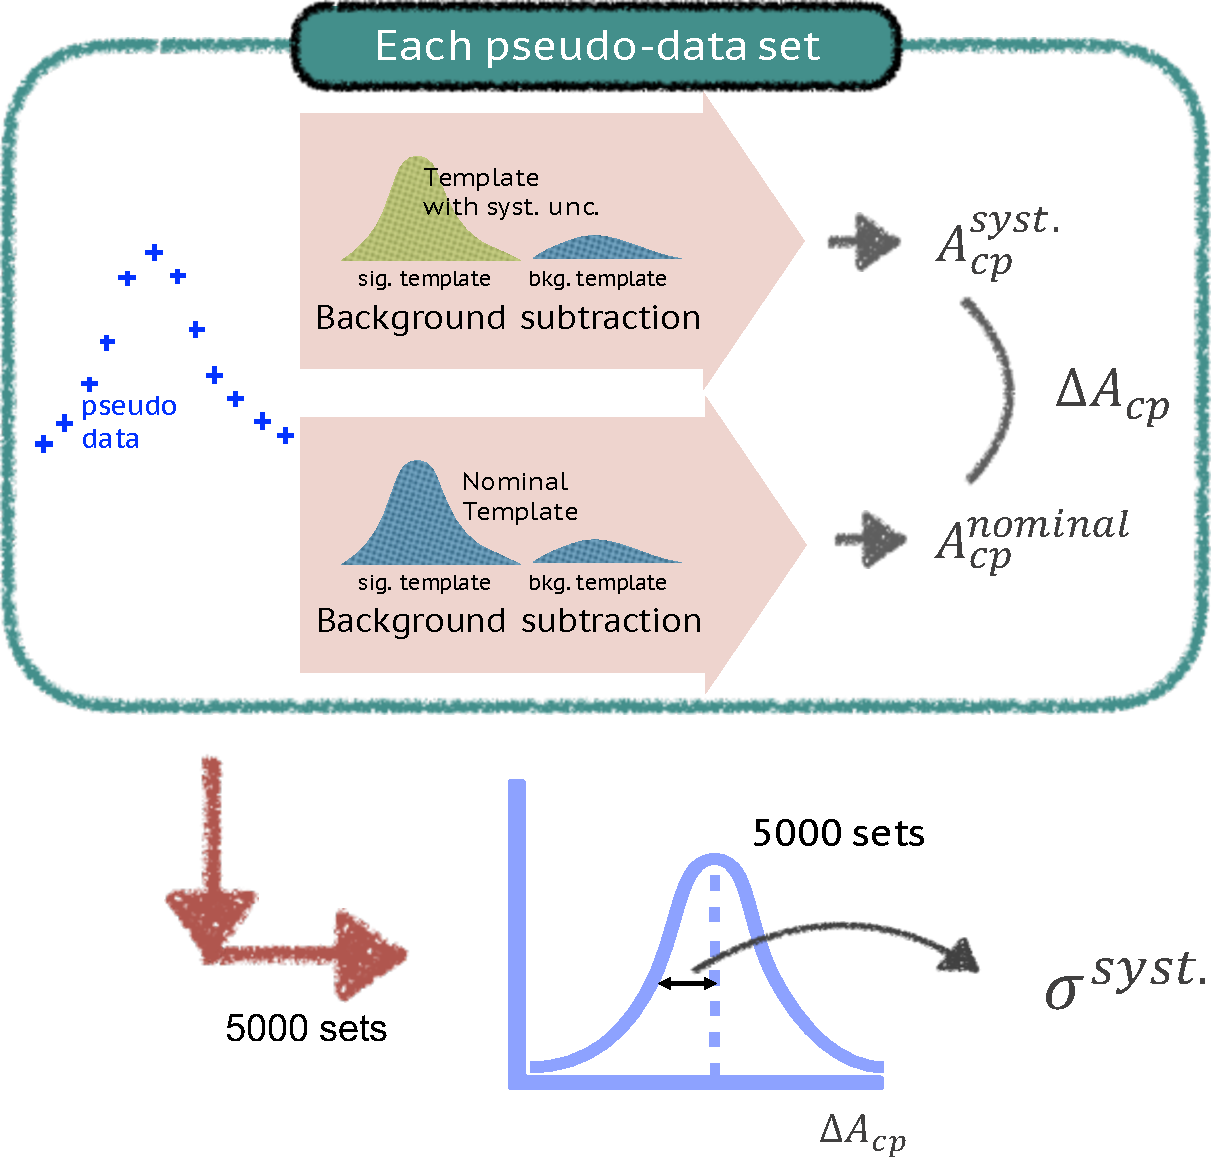
\includegraphics[width=0.85\textwidth]{Figures/SystUnc/approach_syst.pdf}\\
		\caption{Process of measuring systematic uncertainty}
		\label{BkgEst:fig:Bkt_sub}
		\end{figure}
		\FloatBarrier


\FloatBarrier
